% Chapter 6

\chapter{Bilder} % Main chapter title

\label{Bilder} % For referencing the chapter elsewhere, use \ref{Chapter1}

\lhead{\chaptername{} \thechapter{} - \emph{Bilder}} % This is for the header on each page - perhaps a shortened title

%----------------------------------------------------------------------------------------

Der folgende Abschnitt bezieht sich auf den technischen Einsatz von Bildern in einer Gestaltung, Themen wie Ästhetik oder das Finden von passenden Bildern für eine Gestaltung werden hier nicht behandelt.
Diese Themenabgrenzung begründet sich zum Einen mit dem schieren Umfang des Themas Ästhetik und Fotografie, der im Rahmen dieses Projektes nicht abgedeckt werden kann, zum Anderen ist die Abgrenzung eine Folge der Fehleranalyse, in der vor allem technische Mängel beim Einsatz von Bildern auffielen. Weiterhin ist es gerade in einem wissenschaftlichen Studiengang nicht immer möglich, ästhetisch schöne Bilder zu verwenden.

Während der Fehleranalyse fielen vor allem zwei Arten von Fehlern auf: Strecken bzw. Stauchen von Bildern und das Verwenden von verpixelten Bildern.

Im Folgenden sollen die Hauptursachen für diese Fehler identifiziert und Ansätze entwickelt werden, wie diese vermieden werden können. Außerdem gilt es festzustellen ob, und wenn ja wie die erarbeiteten Techniken im Tool interaktiv vermittelt werden können.

\section{Strecken \& Stauchen}
Gestreckte und gestauchte Bilder in einer Gestaltung hinterlassen beim Betrachter einen unprofessionellen Eindruck.
Zwar konnten keine wissenschaftlichen Belege dafür gefunden werden, ab welchem Grad der Verzerrung und wie schnell Menschen ein Bild als verzerrt erkennen, jedoch kann mit einiger Sicherheit davon ausgegangen werden, dass die meisten Menschen ein verzerrtes Bild erkennen, gerade wenn sich im Bild ihnen bekannte Objekte befinden.

Ursache für das Strecken oder Stauchen eines Bildes ist die Veränderung des ursprünglichen Seitenverhältnisses des Bildes beim Skalieren. \\
Als Seitenverhältnis wird das Verhältnis der beiden Kanten eines Bildes zueinander bezeichnet. Obwohl die Berechnung des Seitenverhältnisses an sich in der Praxis eine eher unwichtige Rolle spielt (in der Regel errechnen Programme dieses Verhältnis automatisch), wird sie für das Tool nötig sein, um eine korrekte Skalierung zu überprüfen.
Wie bereits durch die Schreibweise (\textit{4:3}, \textit{16:9}, ...)  angedeutet, lässt sich das Seitenverhältnis berechnen, indem die Breite des Bildes durch die Höhe des Bildes dividiert wird. \\
Für ein Bild mit den Maßen $400px \times 300px$ ergibt sich also ein Seitenverhältnis von \(400 / 300 = 1,33\) bzw. \textit{4:3}.
Beim Skalieren des Bildes sollte also darauf geachtet werden, beide Kanten im gleichen Verhältnis zu skalieren, um das Bild nicht zu strecken oder zu stauchen (s. Abb. \ref{fig:scaling} auf Seite \pageref{fig:scaling})

\begin{figure}[h]
    \centering
    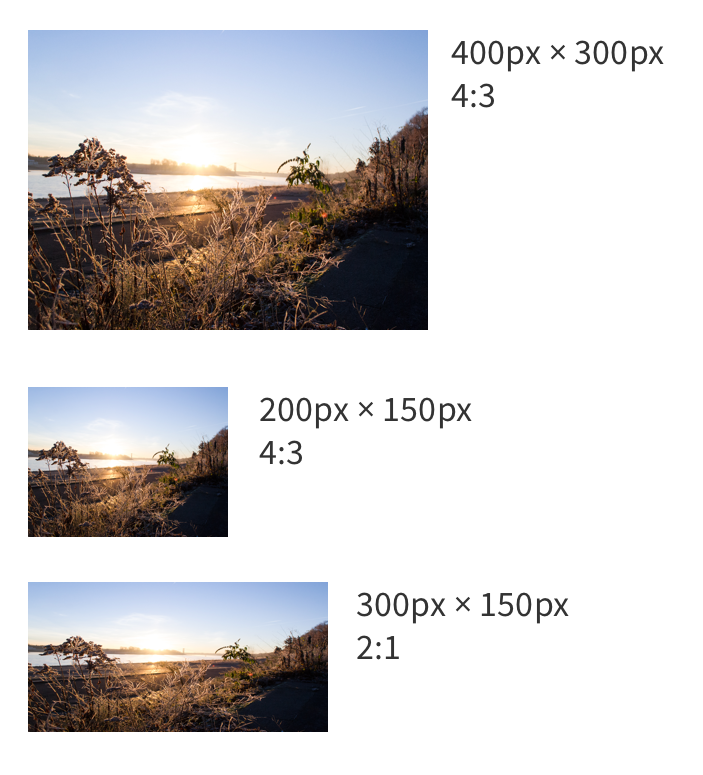
\includegraphics[width=0.8\textwidth]{images/scaling.png}
    \caption{Beispiele für das korrekte und falsche Skalieren eines Bildes}
    \label{fig:scaling}
\end{figure}

Häufig treten Fehler in der Skalierung vor allem dann auf, wenn das Bild eine gegebene Fläche ausfüllen soll, die nicht dem Seitenverhältnis des Originalbildes entspricht.
Ein reines Skalieren des Bildes reicht hier nicht aus, um ein befriedigendes Ergebnis zu erzielen, häufig müssen Teile des Bildes abgeschnitten werden, um die gewünschte Größe zu erreichen.
Welcher Teil des Bildes abgeschnitten wird und welcher erhalten bleibt, ist dabei wiederum eine ästhetische Entscheidung und kann nur in Abhängigkeit vom Bild und der gewünschten Wirkung getroffen werden. Im besten Falle wird die Kernaussage des Bildes durch die Beschneidung nicht verändert. Das Tool könnte dies Beispielhaft mit einigen Bildern demonstrieren.

Grafikprogramme bieten für das Ausführen dieser Aufgabe verschieden Möglichkeiten, sowie das einfache Beschneiden des Bildes oder den Einsatz von Masken. Unter Umständen muss auf solche Programme zurückgegriffen werden, wenn das gewählte Textverarbeitungsprogramm oder der gewählte Editor diese Möglichkeit nicht bietet.

Auch im Web bieten sich hierfür verschiedne Möglichkeiten an. Die meiste Kontrolle über die Ausrichtung des beschnittenen Bildes bringt dabei die Verwendung des Bildes als Hintergrundbild über das CSS-Attribut \textit{background-image} mit sich. Über den Wert \textit{cover} des Attributes \textit{background-size} wird sichergestellt, dass das Bild immer die gewünschte Fläche ausfüllt, ohne dabei gestreckt oder gestaucht zu werden (s. Quellcode \ref{lst:background-iamge} auf Seite \pageref{lst:background-iamge}).

\begin{lstlisting}[caption={Verwendung eines Hintergrundbildes in CSS},label={lst:background-iamge}]
.bg-image {
  width: 300;
  height: 150;
  background-image: url("image/landscape.jpg");
  background-size: cover;
}
\end{lstlisting}

\section{Verpixelte Bilder}
Neben gestreckten und gestauchten Bildern fallen auch verpixelte oder verschwommene Bilder unschön auf und verschlechtern die Qualität einer Gestaltung. Verpixelte Bilder können aus verschiedenen Gründen auftreten, die häufigste Ursache liegt aber in der Skalierung von Bildern über ihre Originalgröße hinaus. 
Da dieses Problem nur bei der Verwendung von Bitmaps auftritt, sei hier kurz angeschnitten, was genau beim Skalieren einer Bitmap geschieht.

Enderle, Kansy und Pfaff definieren Bitmaps oder Raster Graphics wie folgt:

\begin{quote}
Raster graphics — Definition \\
Computer graphics in which a display image is composed of an array of pixels arranged in rows and columns. \cite{enderle2012computer}
\end{quote}

Bitmaps bestehen also aus einem Array von Pixeln, von denen jeder seine eigene Farbe und Position hat.
Beim Skalieren einer Bitmap muss also eine neue Anzahl an Pixeln innerhalb dieses Rasters erzeugt werden. Beim Skalieren nach unten ist dies kein Problem, da benachbarte Pixel zu einem neuen Pixel zusammen gefasst werden und aufgrund des kleineren Bildes für das Menschliche Auge kein Unterschied in der Qualität zu erkennen ist.

Beim Skalieren nach oben müssen jedoch neue Pixel basierend auf der Datengrundlage des Bildes erzeugt werden. Bei der Skalierung nach oben können zwar, ähnlich wie bei der Skalierung nach unten, neue Pixel anhand der vorhandenen errechnet werden, jedoch wird diese Berechnung aufgrund der fehlenden Datengrundlage schnell ungenau und das Bild wirk verschwommen. Nach Möglichkeit sollten Bilder also nicht über ihre Originalgröße hinaus skaliert werden..

Eine weitere Ursache für verpixelte Bilder liegt in der Verwendung von für das Medium unpassenden DPI-Werten. Da dieses Themengebiet sich aber weit von der Sicherung von gestalterischen Grundalgen entfernt soll es hier nicht behandelt werden.

Problematisch gestaltet sich eine interaktive Abbildung der gewonnen Erkenntnisse im Tool, da es sich hierbei eher um handwerkliche Richtlinien handelt, als um Regeln der Gestaltung, die durch einen \textit{Trial \& Error} Ansatz erlernt werden können.